\documentclass[12pt,letterpaper]{hmcpset}
\usepackage[margin=1in]{geometry} 
\usepackage{graphicx}
\usepackage{amsmath}
\usepackage{boxedminipage}
\usepackage{url}
\usepackage{geometry}

%\geometry{tmargin=1.5cm} % To fix some issues with the first paper.

% info for header block in upper right hand corner
\name{ }
\class{Math 45 - Section --- \hspace{20pt}}
\assignment{HW 05}
\duedate{Due: Friday, 2016-04-01}

\newcommand{\pn}[1]{\left( #1 \right)}
\newcommand{\abs}[1]{\left| #1 \right|}
\newcommand{\bk}[1]{\left[ #1 \right]}

\newcommand{\vb}{\mathbf{v}}
\newcommand{\ub}{\mathbf{u}}
\renewcommand{\labelenumi}{{(\alph{enumi})}}

\begin{document}

\problemlist{1, 2, 3, 4, 5}
% 1 %
\begin{problem}[1]
    {\textbf{Leaky bucket:} A bucket in the shape of a cylinder has a
        small hole in its bottom, through which water is leaking. Let $h(t)$ be the height
        of the water in the bucket, $A$ the
        cross-sectional area of the bucket, and $a$ the area of the small
        hole. We want to find how long it will take the bucket to
    empty.}
    \begin{center}
        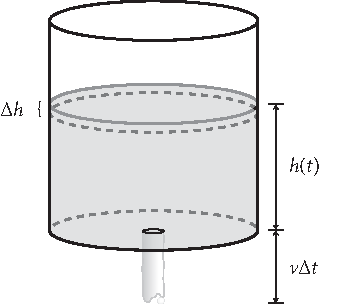
\includegraphics[width=2in]{img/bucket}
    \end{center}
    \begin{enumerate}
        \item Let's assume that the water flows out of the
            bucket laminarly, so that the stream of water looks roughly like a
            cylinder with cross-sectional area $a$ (the same as the hole). Let
            $v(t)$ be the velocity of the water when it exits the bucket. It
            is a fact that
            \[
                a\,v(t)=A\,h'(t).
            \]
            What physical principle is responsible for this fact?
            \textbf{Hint:} In a small unit of time $\Delta t$, the height of the
            water in the bucket falls by $\Delta h$ and the water at the hole
            travels a distance $v(t)\Delta t$, as indicated in the diagram above.
        \item Now let's derive a differential equation for $h(t)$ based on
            conservation of energy. If the height of the water in the bucket
            decreases by $\Delta h$ and the density of the water is $\rho$, the
            net change of potential energy in the system is $\Delta m\, gh=\rho
            A\Delta h\, gh$. Since energy cannot be created or destroyed,
            this decreased potential energy must be converted into kinetic energy.
            The kinetic energy of the same amount of water leaving the bucket is
            $\tfrac{1}{2} \Delta m\, v^2=\tfrac{1}{2}\rho A\, \Delta h\, v^2$.
            Equating these two energies, we get $v^2=2gh$. Using this
            information, derive a differential equation for $h(t)$.
        \item Assume that at $t=0$ the height of the water in the bucket is
            $h_0$. Define $t^{\ast}$ to be the time when the bucket becomes
            empty. Find an expression for $t^{\ast}$.  What is $h(2t^{\ast})$?
            (Make sure your answer is sensible.)\newpage
        \item Suppose that at $t=5$ you observe that the bucket is empty. Is
            it possible to determine \textit{uniquely} how full the bucket was
            at $t=0$? Explain why or why not.
    \end{enumerate}
\end{problem}
\newpage
\begin{solution}
    \null\vfill
\end{solution}
\newpage

% 2 %
\begin{problem}[2]
    For each IVP, what can you say about the interval forward in time from the initial condition in which you can guarantee existence and uniqueness of the solution?  Make sure you explain why your claim is true.   Use dfield\footnote{Use either the Matlab version or the Java version at \url{http://math.rice.edu/~dfield/dfpp.html}} or ODEToolkit\footnote{\url{http://odetoolkit.hmc.edu}} to plot a direction field and solution curve for each IVP.  In a couple of sentences, explain how the solutions you see are or are not consistent with the results of the theorem(s) you applied.  \textbf{You do not have to analytically solve the IVPs.}
    \begin{enumerate}
        \item $(\sin t) y' + y = 2; y(5) = -2$ 
        \item $(t-5) y'+ t y = e^{-t}; y(0) = 1$
        \item  $y'=3y^2; y(2)= 3$
    \end{enumerate}
\end{problem}

\begin{solution}
    \vfill
\end{solution}
\newpage

% 3 %
\begin{problem}[3]
    What linear, second-order, constant-coefficient, unforced DE can have $y(x)=Ce^{-5x}+De^{2x}$ as its general solution? Also, determine the characteristic equation that is consistent with this general solution.
\end{problem}

\begin{solution}
    \vfill
\end{solution}
\newpage

\begin{problem}[4]\begin{enumerate}
    \item Find the solution to the IVP $\ddot{y}+21\dot{y}+20y=0$ with $y(0)=0$, $\dot{y}(0)=19$.
    \item Your answer to (a) is the sum of two exponential terms. Suppose $t>0$. As $t$ increases, which term is negligible and which dominates? Graph your answer to (a) along with the dominant exponential term by itself on the same axes to verify your answer.
\end{enumerate}
\end{problem}

\begin{solution}
    \vfill
\end{solution}
\newpage

\begin{problem}[5]
    In the Resources section on our Sakai site, there is a folder entitled ``ODE Papers'' that contains 10 different research papers that use differential equations in a mathematical model.  Locate the paper whose last digit of year of publication matches the second-to-last digit (before the dash) of your HMC ID. Read that paper to see how the author(s) used ODEs to create a mathematical model. You don't have to read the paper thoroughly (unless you want to), you only need to skim it as much as you need to gather the answers to the following questions. Don't worry if you can't understand every piece of the article---just try your best.
    \begin{enumerate}
        \item What is the main question that the author(s) wanted to address through their mathematical model?
        \item Do the authors describe how they derived the differential equation(s) used in the paper?  If so, in which paragraph did they do so?
        \item As best as you can determine, what are the governing principles that were used to derive the differential equation(s) used in the paper?  (For example, Newton's Second Law, or conservation of energy, or conservation of cancer cells.)
        \item As best as you can determine, what is one simplifying assumption that was used in the creating the mathematical model?  Did the authors justify that simplification, and if so, how?
        \item Describe the differential equations that were used in the paper. Is it a single differential equation or a system of differential equations? What order? Linear? Autonomous? Driven (if linear)? 
        \item As best as you can determine, how did the authors analyze the differential equations?  They did come up with an analytical solution?  Did they use a computer to calculate numerical solutions?
        \item As best as you can determine, what is the conclusion is reached about the main question (that you wrote in part a) raised in the paper?
    \end{enumerate}
    Feel free to browse the other papers if you find them interesting!
\end{problem}
\newpage
\begin{solution}
    \null\vfill
\end{solution}
\end{document}
